% !TEX program = xelatex
%% Requires compilation with XeLaTeX or LuaLaTeX
\documentclass[10pt,xcolor={table,dvipsnames},t]{beamer}
\usepackage{biblatex}
\usepackage{caption}
\setbeamertemplate{caption}[numbered]
\addbibresource{reference.bib}
\usepackage{hyperref}
\hypersetup{ 
pdfpagemode=FullScreen,  
colorlinks=true,linkcolor=blue}

\usetheme{UCBerkeley}

\title[Your Short Title]{STMC coding team training}
\subtitle{Lesson 0: Introduction}
\author{TSAI Yun Chen}
%\institute{}
\date{\today}

\begin{document}

\begin{frame}
  \titlepage
\end{frame}

% Uncomment these lines for an automatically generated outline.
%\begin{frame}{Outline}
%  \tableofcontents
%\end{frame}

\section{What is programming}

\begin{frame}{To begin with...\\\enspace\\ What do you think of when talking about programming?}
  
\end{frame}

\begin{frame}{What is programming?}

  \begin{itemize}
    \item A \textbf{computer program} is a collection of instructions that can be executed by a computer to perform a specific task \cite{enwiki:Computer_program}.
    \item Tell computer what to do and how to response to input and produce outputs
    \item Similar to writing an article, you need to follow a few rules
  \end{itemize}
  \begin{table}[h!]
    \centering
    \begin{tabular}{|c|c|}
      \hline
      writing&coding\\
      \hline
      grammar&syntax\\
      content&logic/algorithm\\
      organization&structure and indentation\\
      \hline
    \end{tabular}
  \end{table}

\end{frame}

\begin{frame}{Examples of computer programs}
  \begin{itemize}
    \item Web browser
    \item Computer games
    \item Mobile applications 
    \item Operation system (e.g. Windows, Linux, Unix, etc.)
    \item Productivity software (e.g. Word, PowerPoint, Excel, etc.)
  \end{itemize}
\end{frame}

\section{Why programming}
% \begin{frame} {Why learning programming?}
%   \begin{columns}
%     \column{0.6\textwidth}
%     \begin{itemize}
%       \item Programming is \textit{everywhere}!
%       \item Science:
%       \begin{itemize}
%         \item Computer simulations
%         \item Automatic data collection for experiments 
%         \item Analysis of huge amount of data \\(Fig.~\ref{fig:eht_blackhole})
%         \item Develop more efficient algorithms
%         \item Develop state-of-the-art AI 
%       \end{itemize}
%     \end{itemize}

%     \column{0.4\textwidth}
%     \begin{figure}
%       
\includegraphics[width=0.6\textwidth]{img/blackhole.png}
%       \caption{The first image of black hole is obtained by analysing over 4.5 petabyte of data \cite{westerndigital:EHT_blackhole}. An impossible task without programming (Source: \href{https://www.nasa.gov/mission_pages/chandra/news/black-hole-image-makes-history}{NASA}).}
%       \label{fig:eht_blackhole}
%     \end{figure}
%   \end{columns}
  
% \end{frame}

% \begin{frame}{Why learn programming?}
%   \begin{columns}
%     \column{0.6\textwidth}
%     \begin{itemize}
%       \item Engineering
%       \begin{itemize}
%         \item Run code to calculate forces and stresses when designing building or aircrafts
%         \item Engineering fluid simulation
%         \item Game development
%         \item Mobile app development
%       \end{itemize}
%     \end{itemize}

%     \column{0.4\textwidth}
%     \begin{figure}
%       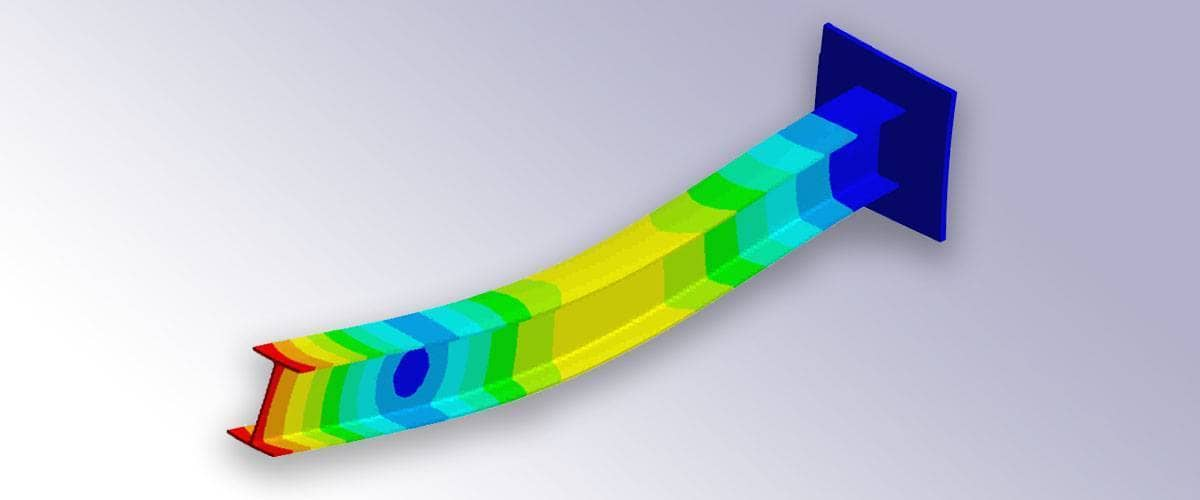
\includegraphics[width=0.9\textwidth]{img/euler-beam.jpg}
%       \caption{Simulation of beam oscillating freely in one end (Source: \href{https://www.featool.com/tags/beam/}{FEATool})}
%       \label{fig:euler_beam}
%     \end{figure}
%   \end{columns}
% \end{frame}

\subsection{How code works}

\begin{frame}{Cool, but what is INSIDE a computer program?}
  \begin{columns}
    \column{0.6\textwidth}
    \begin{itemize}
      \item Computer programs consist of \textbf{machine code} that are made up of 0s and 1s
      \item It's groups of 0s and 1s that represent instructions directly executable by computer.
      \item Different operation systems (e.g. windows vs Mac) have dfferent set of instruction.
    \end{itemize}
  

    \column{0.4\textwidth}
    \begin{figure}
      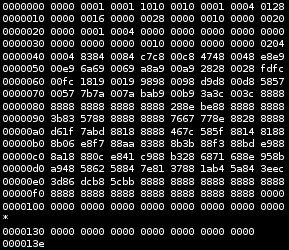
\includegraphics[width=0.8\textwidth]{img/machine-code.png}
      \caption{Machine code (Source: \href{https://bit.ly/3sQendj}{https://bit.ly/3sQendj})}
      \label{fig:machine_code}
    \end{figure}
  \end{columns}

\end{frame}

\begin{frame}{But... We don't speak machine code right?}
  \begin{columns}
    \column{0.6\textwidth}
    \begin{itemize}
      \item In order to communicate to machine more efficiently, people invented the \textbf{high level language}
      \item Examples: C/C++, Java, Python, Ruby, R, PHP, etc.
      \item It is composed of word and symbol that are used in daily life (e.g. if, while, y=x+c etc.)
      \item Code written in high level language are usually called \textbf{source code}
    \end{itemize}
  

    \column{0.4\textwidth}
    \begin{figure}
      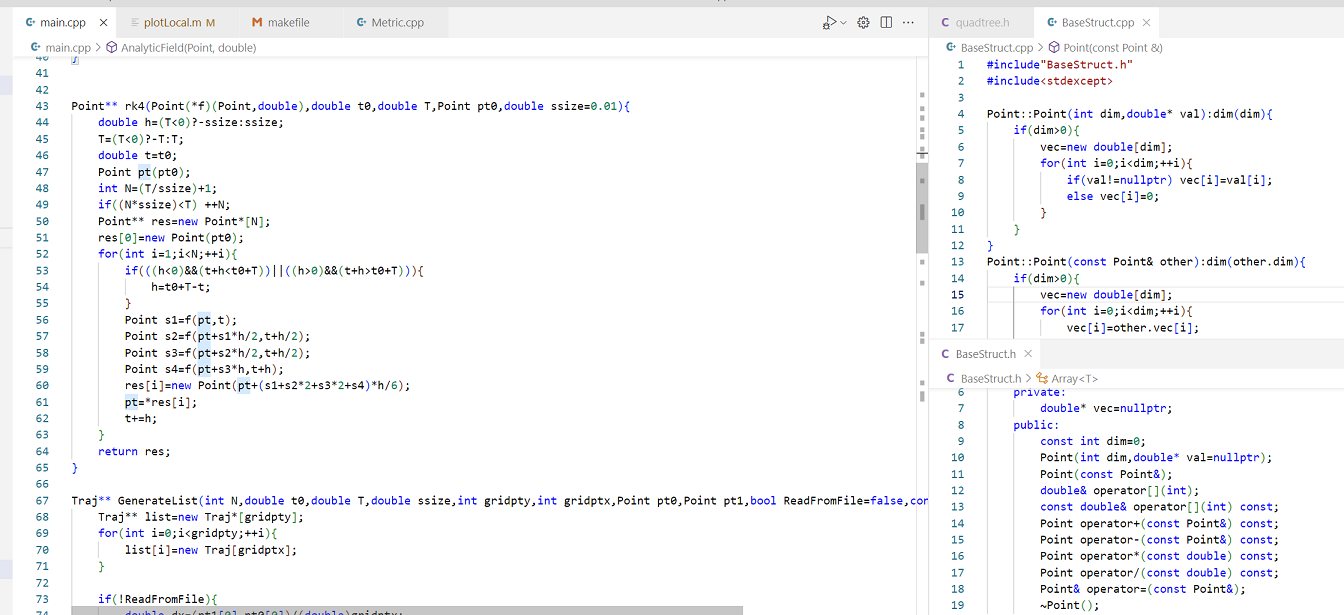
\includegraphics[width=0.9\textwidth]{img/C++code.png}
      \caption{Source code in C++ (Source: me)}
      \label{fig:python_code}
    \end{figure}
  \end{columns}
  
\end{frame}

\begin{frame}{Compiler: Translate source code to machine code}
  \begin{columns}
    \column{0.6\textwidth}
    \begin{itemize}
      \item Like we don't speak machine code, machine don't know how to interpret source code.
      \item We need a ``translator'' to do the translation,from source code to machine code
      \item That's what a \textbf{compiler} do
      \item The compiled result is called an \textbf{executable}, which has the file extension of \texttt{.exe} in Windows
    \end{itemize}
  

    \column{0.4\textwidth}
    \begin{figure}
      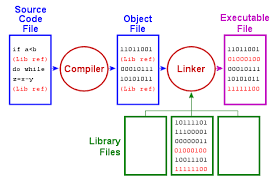
\includegraphics[width=0.9\textwidth]{img/compiling.png}
      \caption{Compiling source code to executables (Source: \href{https://bit.ly/3sQendj}{https://bit.ly/3sQendj})}
      \label{fig:compiling}
    \end{figure}
  \end{columns}
  
\end{frame}

\begin{frame}{Some other solution}
  While machine code is machine dependent (since they have different instruction set), therefore we need to re-compile the source code everytime we change the machine we work on, below are some method to avoid this.
  \begin{block}{1. Two-step conversion}
    \begin{itemize}
      \item Instead of directly translating the source code into machine code, we can first translate it into the instruction needed
      \item upon running the program, we then translate the instruction to the machine code needed
      \item Java works in this way (thats why you need to install Java on your computer before playing Minecraft)
    \end{itemize}
  \end{block}
\end{frame}

\begin{frame}{Some other solution}
  \begin{block}{2. Intepreter}
    \begin{itemize}
      \item For some programming language (like Python), the high level instructions are compiled line-by-line during runtime
      \item The software that do that is called an \textbf{interpreter} instead of a compiler
    \end{itemize}
  \end{block}
\end{frame}

\begin{frame}{Let's move on to write our first program ... }
  
\end{frame}
\begin{frame}[allowframebreaks]{Reference}
  \printbibliography
  %\bibliography{./reference.bib}
\end{frame}
\end{document}
